\chapter{Modelling}
\section{Parameters for testing}
For testing, parameters used in testing codes (\autoref{TestCodes}), could be assumed as \autoref{testpara}:
\begin{center}
    \begin{longtable}{cccc}
        \caption{Parameters for testing}
        \label{testpara} \\
            \hline
            Parameters & Values     & Units                   & Meanings   \\
            \hline
            \endfirsthead
            \hline
            Parameters & Values     & Units                   & Meanings   \\
            \hline
            \endhead
            \cline{1-4}
            \multicolumn{4}{c}{Variable}                                                                                \\
            \cline{1-4}
            time       &0.1;1;10;100        & $h$                       & given time \\
            num\_iter  & 30;50         &                         & limitation of   iterations                                    \\
            \cline{1-4}
            \multicolumn{4}{c}{Grid} \\
            \cline{1-4}
            sx         & 3          &                         & x position of the   start point                               \\
            sy         & 3          &                         & y position of the   start point                               \\
            gx         & 47         &                         & x position of the   goal point                                \\
            gy         & 47         &                         & y position of the   goal point                                \\
            xcol       & 50         &                         & number of columns                                             \\
            yrow       & 50         &                         & number of rows                                                \\
            dist       & 1000       & $m$                       & distance between   neighbour nodes                            \\
            \cline{1-4}
            \multicolumn{4}{c}{Ship}                                                                                          \\
            \cline{1-4}
            L          & 200        & $m$                       & length of this ship                                           \\
            Lwl        & 195        & $m$                       & length of water line                                          \\
            Lbwl       & 38         & $m$                       &\makecell[c]{length of the bow on the water line \\to 95\% of maximum beam}      \\
            Los        & 196.5      & $m$                       & length over surface                                           \\
            B          & 33         & $m$                       & beam                                                          \\
            TF         & 11.6       & $m$                       & draft of fore   propeller                                     \\
            TA         & 11.4       & $m$                       & draft of aft   propeller                                      \\
            CB         & 0.855      &                         & block coefficient                                             \\
            S          & 10500      & $m^2$    & wetted surface                                                \\
            Axv        & 1600       & $m^2$    & \makecell[c]{area of maximum transverse section\\exposed to the wind}      \\
            Dp         & 7          & $m$                       & propeller diameter                                            \\
            NRud       & 1          &                         & nubmer of rudder                                              \\
            NBrac      & 1          &                         & number of brackets                                            \\
            NBoss      & 1          &                         & number of bossings                                            \\
            NThr       & 1          &                         & nubmer of side   thrusters                                    \\
            \cline{1-4}
            \multicolumn{4}{c}{Constant}                                                                                      \\
            \cline{1-4}
            rho\_air   & 1.293      & $kg/m^3$ & density of air                                                \\
            rho\_sea   & 1025       & $kg/m^3$ & density of sea                                                \\
            nu\_sea    & 1.1395E-06 & $m^2/s$  & viscosity of sea                                              \\
            g          & 9.81       & $m/s^2$  & gravitational   acceleration                                 
    \end{longtable}
\end{center}
\section{Tests and results}
\label{TestResults}
The aim of this project is to find the optimum velocity and the efficient path under this speed, which would lead to minimum cost. So, for this aim, these tasks are set as that a ship needs to drive from the start point (3,3) to the goal point (47,47) within a given time and number of iterations. Variables for these 5 tests are shown as:
\begin{table}[H]
    \begin{center}
        \caption{Tests and results:}
        \label{T&R}
        \begin{tabular}{cccc}
            \hline
            Test & Given time[$h$] & Number of iterations & results \\ 
            \cline{1-4}
            1 & 0.1 & 30 & success\\
            2 & 1 & 30 & success\\
            3 & 10 & 30 & success\\
            4 & 100 & 30 & failure \\
            5 & 100 & 50 & success\\
            \hline
        \end{tabular}
    \end{center}
\end{table}
\begin{table}[H]
    \begin{center}
        \caption{Results of successful tests:}
        \label{VandC}
        \begin{tabular}{cccc}
            \hline
            Test & Optimal Velocity[$knot$] & Minimum Total Cost[$MJ$] & Paths \\ 
            \cline{1-4}
            1 & 480.603 & $2.7*10^{62}$ & \autoref{Test 1} \\
            2 & 48.600 & $5.4*10^8$ & \autoref{Test 2} \\
            3 & 5.454 & 97287.277 & \autoref{Test 3} \\
            5 & 0.648 & 9348.747 & \autoref{Test 5} \\
            \hline
        \end{tabular}
    \end{center}
\end{table}
\begin{figure}
    \centering  
	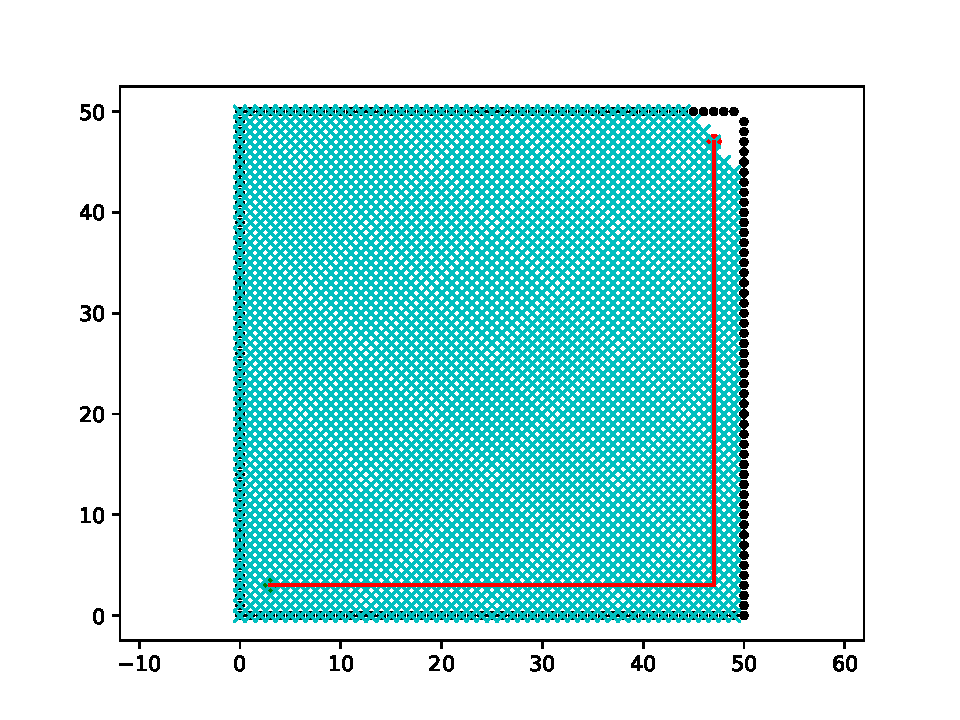
\includegraphics[width=0.9\linewidth]{0.1.pdf}  
	\caption{Result of Test 1}
    \label{Test 1}
\end{figure}
\begin{figure}
    \centering  
	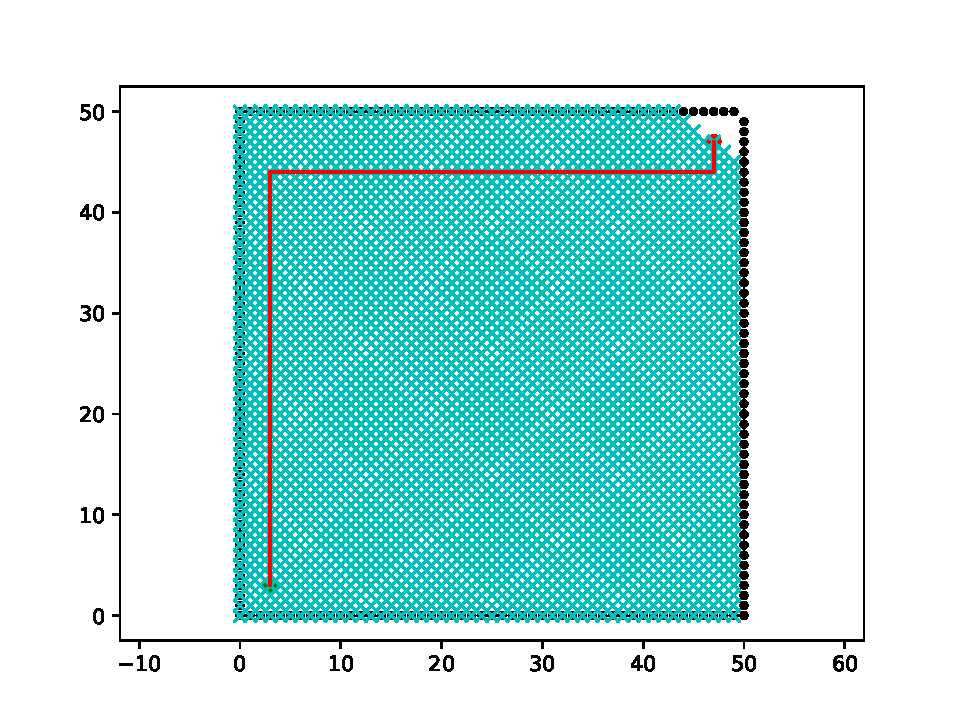
\includegraphics[width=0.9\linewidth]{1.pdf}  
	\caption{Result of Test 2}
    \label{Test 2}
\end{figure}
\begin{figure}
    \centering  
	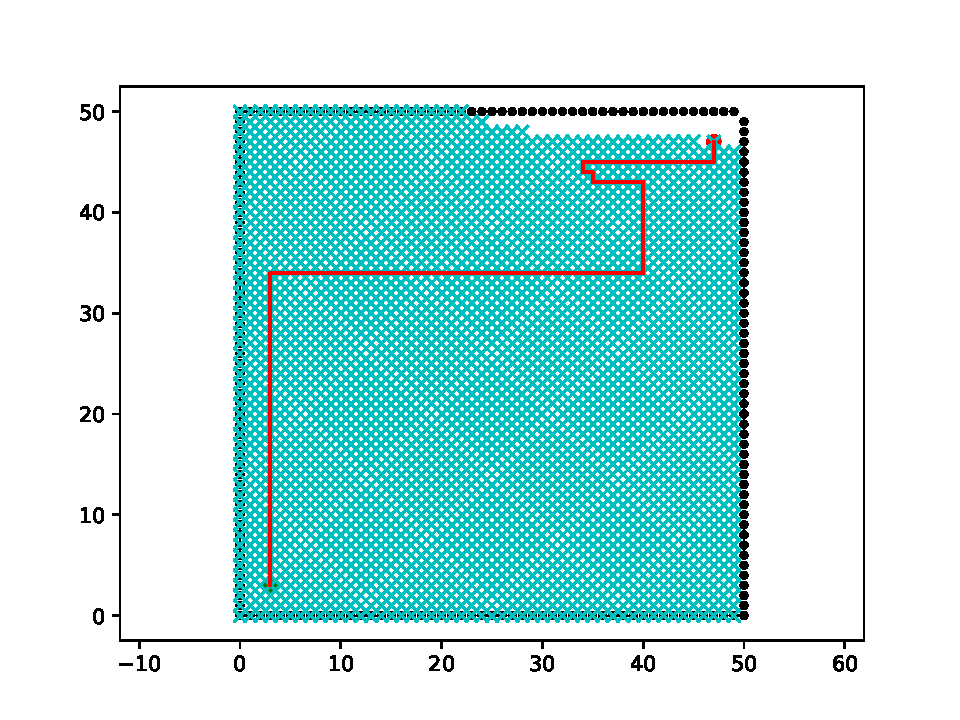
\includegraphics[width=0.9\linewidth]{10.pdf}  
	\caption{Result of Test 3}
    \label{Test 3}
\end{figure}
\begin{figure}
    \centering  
	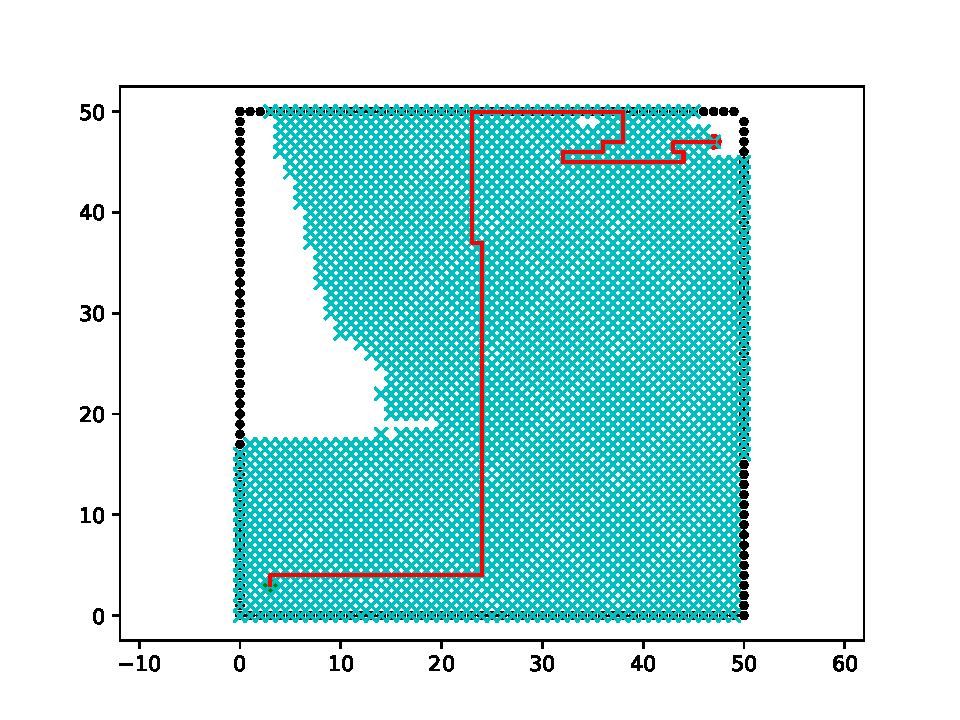
\includegraphics[width=0.9\linewidth]{100.pdf}  
	\caption{Result of Test 5}
    \label{Test 5}
\end{figure}
\noindent Results of test 1 is shown in \autoref{VandC} and \autoref{Test 1}, the ship heading east firstly. This is because excessive speed would make the influence of heading angles greater, in which case all costs caused by eastward movements are cheaper than that of northward movements. Results of test 2 is shown in \autoref{VandC} and \autoref{Test 2}, where the path of test 2 is similar than that of first task. 
\\Owing to the impact of moving too fast, the cost between two neighbour nodes is so big that the ship would prefer to go straight to the target point like the first two tests. The optimum path causing minimum costs would always be found in shortest paths.
\\As is shown in the \autoref{VandC}, the smaller the ship speed is, the lower the cost between neighbour nodes would be, so is the total cost. If the cost of more steps would be cheaper, shortest paths with high costs would be given up, which could be proved by results of 3rd test and 5th test (\autoref{Test 3} and \autoref{Test 5}). On the other side, for each velocity, the increasing path length need take more time, which may make this task not finished in given time. Moreover, the algorithm iterates from the minimum speed, and  when following the shortest path, the lower limit speed for completing the task on time is the smallest. This low limit is increasing with the growing path length. So if the starting velocity is low enough to avoid the shortest path, it would need more iterations to find velocity which reach the new lower speed limit. That is why test 4 fails and test 5 succeeds with more iterations.
\\As it states above, the incresement of cost is closely related with the growth of speed and the algorithm iterates from the minimum speed. So, normally, the optimal velocities would be the minimum velocity which reach the lower speed limit, which is true for first 3 tests. However, when the speed is low, the ocean weather would play a more important role in resistance generation. So, the minimum velocity may not be the optimum velocity any more, which is proved in test 5. The optimum velocity in test 5 is the second minimal velocity under which this ship could arrive the goal point with in the given time.